\documentclass[a4paper,11pt]{article}
\usepackage[a4paper, margin=3cm]{geometry}
\usepackage[spanish]{babel}%Para el español
\usepackage[utf8]{inputenc}%para los acentos	
\usepackage{amsmath,amssymb,amsfonts,amsthm}
\usepackage{graphicx}
\usepackage{lmodern}
\usepackage[T1]{fontenc}
%----------------------------
\usepackage{xcolor}
\usepackage{listings}

\lstset{
	language=Octave,
	basicstyle=\small\ttfamily,
    keywordstyle=\bfseries\color[rgb]{0,0,1},
    commentstyle=\color[rgb]{0.13,0.54,0.13},
    %0.133333 0.545098 0.133333
    stringstyle=\ttfamily\color{red!50!brown},
	literate=%
	{á}{{\'{a}}}1
    {é}{{\'{e}}}1
    {í}{{\'{i}}}1
    {ó}{{\'{o}}}1
    {ú}{{\'{u}}}1
    {ñ}{{\~{n}}}1
    {<}{{$<$}}1
    {>}{{$>$}}1
    {_}{{\_}}1,    
    frame=single,
    %inputencoding=utf8,
	%extendedchars=false,
	%upquote=true,
    breaklines=true,
    postbreak=\raisebox{0ex}[0ex][0ex]{\ensuremath{\color{red}\hookrightarrow\space}},
}
\usepackage{textcomp}%me dejó usar el simbolo de grados (°)
\usepackage{gensymb}%me dejó usar \degree para las fórmulas
\usepackage{subfig}%me dejó modificar la distancia de las epigrafes.
\usepackage{float}%me dejó fijar la posicion de las impagenes
\usepackage{footnote}
\makesavenoteenv{tabular}
\makesavenoteenv{table}
\usepackage[font=scriptsize,labelfont=bf]{caption}
%\usepackage[spanish,activeacute]{babel}
\graphicspath{{Imagenes/}}
\captionsetup{belowskip=12pt,aboveskip=4pt}


\title{Sistemas de Control I \\ Monografía: 
\\Implementación de sistema de control automático para regulación de la intensidad lumínica\\}

\author{\\Alumno:Morales Esteban Andrés Matrícula:35104714\\
	  Alumno:Salamandri Santiago Matrícula:33414224\\
	  Alumno:Uboldi Marino Matrícula:35258183\\
	  Docente:Ing. Mathe Ladislao			.}
\begin{document}
% genera el titulo
\maketitle
\newpage
% inserta la table de contenidos
\tableofcontents
\newpage
\section{Descripción del problema}
En el prsente trabajo se describirá el proceso de desarrollo de un sistema de control automático para regular la intensidad luminica en una habitáculo.
En un enfoque inicial se plantea un sistema de lazo abierto conformado por 4 componentes principales
\begin{itemize}
	\item Potenciómetro (Resistencia Variable)
	\item Arduino UNO
	\item Circuito Dimmer (Corte Alterna)
	\item Lámpara de filamento incandescente
\end{itemize}

\begin{figure}[H] % Example image
	\center{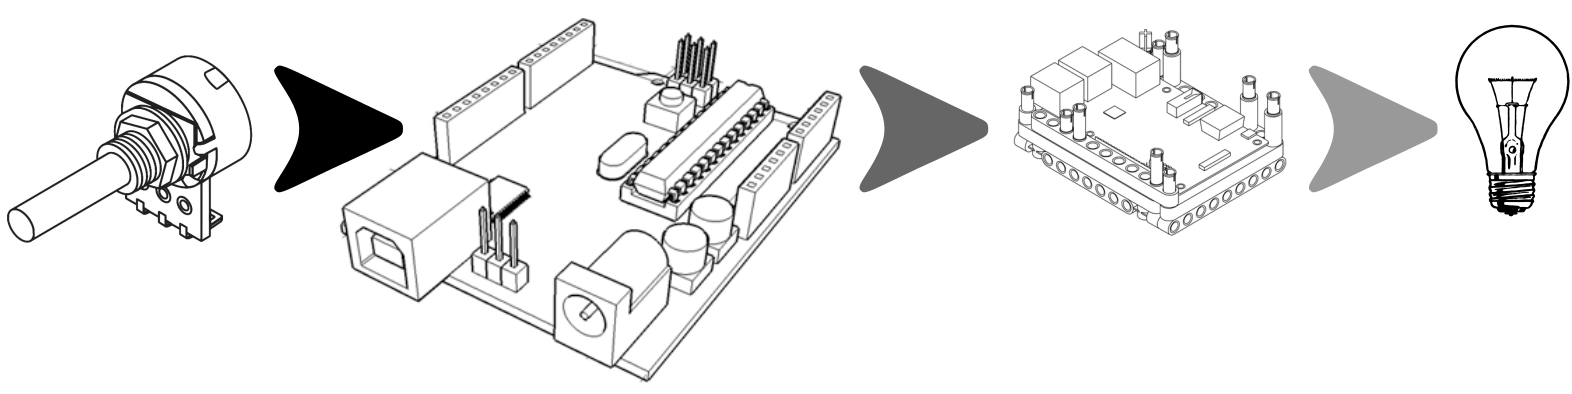
\includegraphics[width=0.9\linewidth]{remake/esquema_ilustrativo.png}}
	\caption{Esquema ilustrativo.}
	\label{fig:esquema_ilustra}
\end{figure} 

En una instancia posterior se incorporará al diseño original un sensor LDR (Light Diode Resistense) de luminosidad para medir el nivel de iluminacion proporcionado por la lampara y de esta manera ofrecer un punto de retroalimentación al sistema inicial. 
\\
Se debe mencionar que el sistema deberá ser capáz de soportar perturbaciones exteriores, como ser la apertura de ventanas o alguna sombra que pueda producirse por distinatas causas, que pueden provenir por el paso de una persona, o de nubes.

%TODO revisar valores. Me parece que la determinación del rango de control se realiza en la etapa de analisi temporal en lazo abierto
La entrada del sistema sera 0V a 10V, que se relacionaran con la salida de forma lineal. El rango de salida del sistema sera de 0lm a 1000lm. Se seleciconara una entrada deseada, por ej 8V al que le corresponde una salida de 800lm, y el sistema debera ser capaz de mantener la salida correspondiente, a pesar de las perturbaciones consideradas.

\subsection{Potenciómetro}
Una resistencia variable utilizada a modo de divisor de tensión permitirá fijar un nivel de control.
\begin{figure}[H] % Example image
	\center{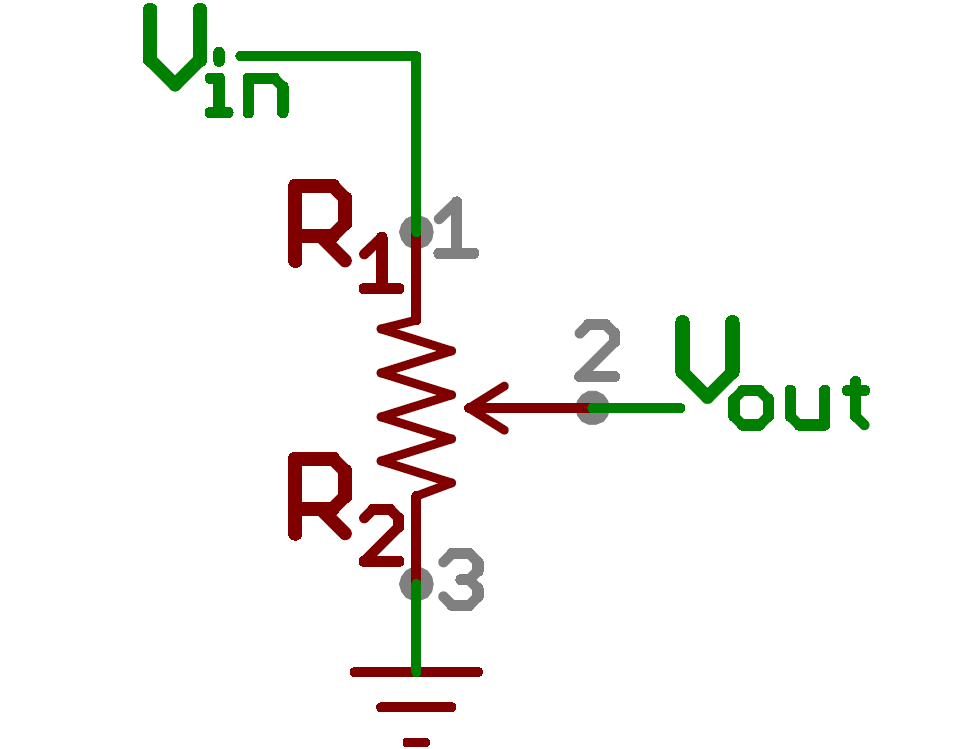
\includegraphics[width=0.3\linewidth]{remake/pote_divisor.png}}
	\caption{Esquema circuito potenciometro.}
	\label{fig:potenciometro}
\end{figure} 

\subsection{Arduino Uno}
Una placa de prototipado digital que incluye un microcontrolador de la marca Atmel ATmega328 será utilizada para medir la señal de ajuste del potenciómetro y permitirá generar las señales de control para el circuito de dimmerización.\\
El microcontrolador funciona por defecto a una velocidad de reloj de 16Mhz lo que se traduce en un tiempo de ejecución de instrucción de aproximadamente 25 ns.\\
Utilizando la librería en C oficial de arduino se consiguen lecturas del ADC cada 100 us y lecturas digitales con una demora de 5 us en promedio por lo que deberán contemplarse dichas demoras en el análisis de las respuestas temporales de cada bloque si fuesen significativas.

\subsection{Dimmer}
Circuito electrónico capaz de detectar cruzes por cero de una señal alterna para los que generará una señal de niveles digitales y corta duración preparada para ser medida.\\
Al mismo tiempo el circuito ofrece una etapa de recorte de la señal alterna de entrada mediante el empleo de un TRIAC.\\
A continuación se muestra un esquema ilustrativo del circuito a ser empleado.

\begin{figure}[H] % Example image
	\center{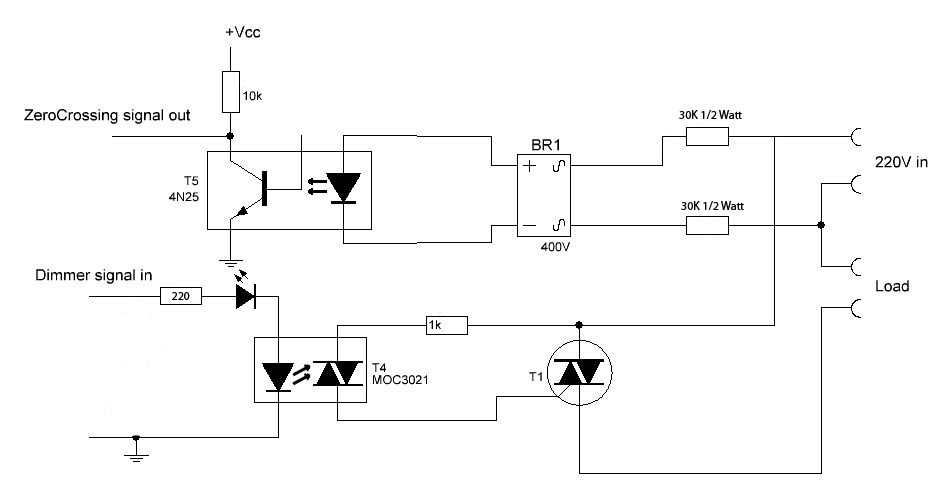
\includegraphics[width=0.8\linewidth]{remake/001__circuito_dimmer.jpg}}
	\caption{Esquema circuito dimmer.}
	\label{fig:dimmer}
\end{figure} 
 
 El efecto de la polarización de la compuerta del TRIAC T1 produce una deformación o corte de la señal alterna original. Tal efecto puede observarse en la forma de onda percibida por la lámpara.
 
 \begin{figure}[H] % Example image
 	\center{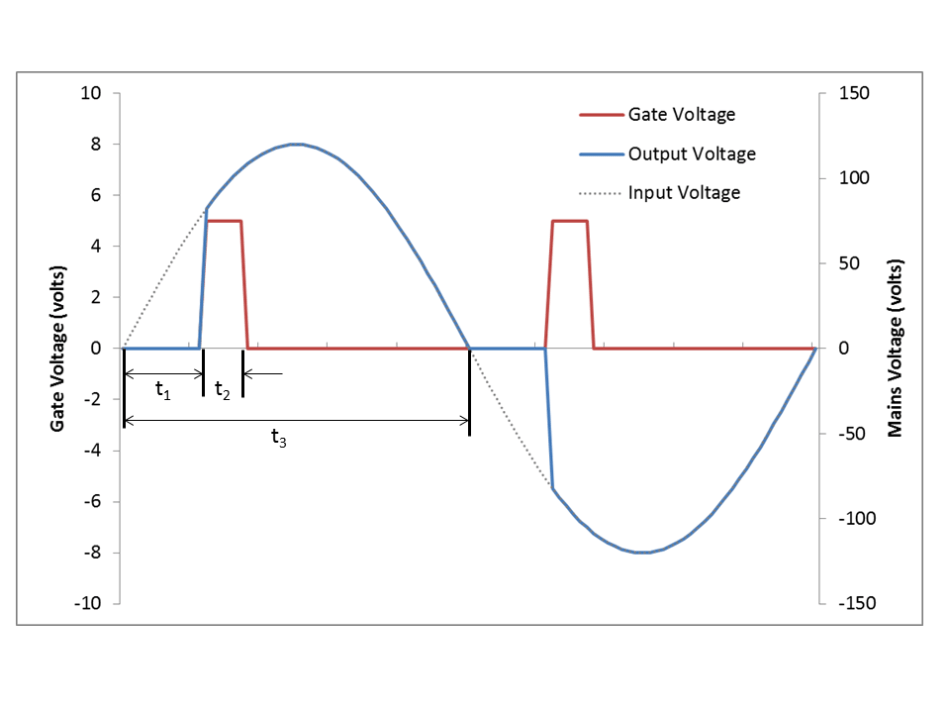
\includegraphics[width=0.7\linewidth]{remake/003__gate_chopped.png}}
 	\caption{Principio de acción sobre la señal original.}
 	\label{fig:gate_chopped}
 \end{figure} 
 
\begin{figure}[H] % Example image
	\center{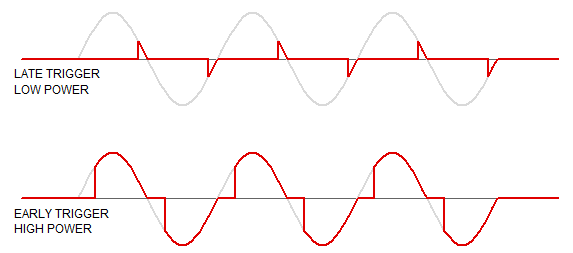
\includegraphics[width=0.7\linewidth]{remake/004__chopped_examples.png}}
	\caption{Ejemplos de deformación de la señal original.}
	\label{fig:chopped_examples}
\end{figure} 
 
 Como puede observarse de la acción de dimmerización la señal deformada cambia con los rertrasos introducidos por los componentes del circuito de dimmer.\\
 Los valores relevantes para este caso se toman en consideración:

\begin{itemize}
	\item Índice de conmutación TRIAC: 20 V/us
	\item Retardo por excitación de compuerta: 2 us
\end{itemize}

\textbf{PEOR ESCENARIO}
$$\widehat{V}_{RED} = 311v$$
$$t_{CONM} = \frac{1}{20}\frac{\mu s}{v}\times 311v$$
$$t_{CONM} = 15,55\mu s$$
$$t_{TOTAL} = 2\mu s + 15,55\mu s$$
$$t_{TOTAL} = 17,55\mu s$$

Sin embargo los efectos del cambio de $V_{RMS}$ aparente se verán completos una vez que termine el ciclo de alterna

$$F_{RED}=50Hz$$
$$T_{RED}=20\mu s$$

\subsection{Lámpara}
El diseño planteado sólo funcionará para lámaparas de filamento incandescente.
Según las especificaciones ofrecidas por OSRAM.
Para alcanzar el 90\% de la iluminación tabulada se requerirá un $t_{REAC}=250ms$
Si se supone la respuesta exponencial entonces 

\begin{align*}
& 90~\text{\small \% } \,\rule[2.5pt]{16pt}{0.5pt}\,
20~\text{\small ms}\\
& 63,2~\text{\small \%} \,\rule[2.5pt]{16pt}{0.5pt}\,
~\text{\small $\tau$}
\end{align*}
$$\tau = 175,5ms$$

\section{Planteo Inicial: Sistema sin Realimentación}
Teniendo en cuenta las consideraciones anteriores puede reducirse el planteo del sistema con el siguiente diagrama de bloques.

\begin{figure}[H] % Example image
	\center{
\includegraphics[width=0.7\linewidth]{remake/005__sistema_sin_retro.png}}
	\caption{Planteo sistema sin realimentación.}
	\label{fig:sistema_sin_retro}
\end{figure} 
Para convertir el esquema en un sistema de control automático es necasario incorporar un componente de retroalimentación, un detector de errores o comparador.

\begin{figure}[H] % Example image
	\center{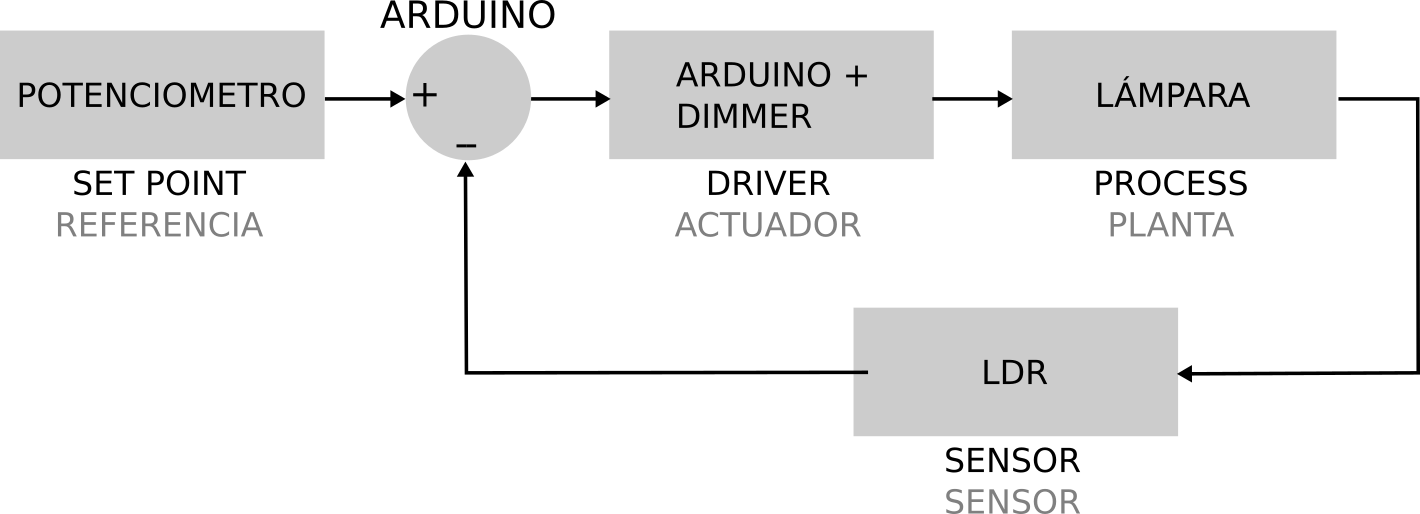
\includegraphics[width=0.7\linewidth]{remake/006__sistema_con_retro.png}}
	\caption{Planteo sistema con realimentación.}
	\label{fig:sistema_con_retro}
\end{figure} 
\subsection{Sensor}
Como componente de lazo de feedback se eligió una Light Dependant Resistance (LDR) configurada en una maya con divisor de tensión es posible conseguir un rango de voltages adecuados.

La respuesta de tiempos de reacción de este dispositivo es asimétrica, esto es para el escenario que contempla la transición LUZ $\rightarrow$ OSCURIDAD TOTAL la variación de la resistencia es inversamente exponencial.
En este caso según la documentación del fabricante el tiempo que tarda en alcanzar el máximo valor para la resistencia interna es de 78ms entonces:
\begin{align*}
& 100~\text{\small \% } \,\rule[2.5pt]{16pt}{0.5pt}\,
78~\text{\small ms}\\
& 63,2~\text{\small \%} \,\rule[2.5pt]{16pt}{0.5pt}\,
~\text{\small $\tau$}
\end{align*}
$$\tau = 50ms$$

El caso inverso atiende el escenario OSCURIDAD TOTAL $\rightarrow$ LUZ la respuesta de la variación de resistencia interna es más que exponencial con una reducción a 0 en menos de 8ms.

Por esta razón se contempla solo el retardo anterior.

\subsection{Funciones de Transferencia}
\subsubsection{ACTUADOR}
$$FT_{Actuador} =\frac{\frac{OUTPUT_{MAX}}{INPUT_{MAX}}}{1+\tau_{BLOQUE}\times s}$$
$$=\frac{\frac{220}{10}}{1+0,02 s}=\frac{22}{1+0,02 s}=\frac{22}{0,02(50+s)}$$
$$FT_{Actuador} = \frac{1100}{s+50}$$

\subsubsection{PLANTA}
$$FT_{Planta} =\frac{\frac{OUTPUT_{MAX}}{INPUT_{MAX}}}{1+\tau_{BLOQUE}\times s}$$
$$=\frac{\frac{1000}{220}}{1+0,2 s}=\frac{4,54}{1+0,02 s}=\frac{4,54}{0,2(5+s)}= \frac{22,7}{s+5}$$
$$FT_{Planta} = \frac{23}{s+5}$$

\subsubsection{SENSOR}
$$FT_{Sensor} =\frac{\frac{OUTPUT_{MAX}}{INPUT_{MAX}}}{1+\tau_{BLOQUE}\times s}$$
$$=\frac{\frac{10}{1000}}{1+0,05 s}=\frac{0,01}{1+0,05 s}=\frac{0,01}{0,05(20+s)}$$
$$FT_{Actuador} = \frac{0,2}{s+20}$$

\section{Funcion de Transferencia de Lazo Abierto}
Utilizando las funciones de transferencia previamente calculadas, se obtiene la funcion de transferencia de lazo abierto del sistema:
$$FT_{LA}=FT_{Actuador} \times FT_{Driver} \times FT_{Planta} \times FT_{Sensor} $$
$$FT_{LA}=\frac{1}{0.001386s^3 + 0.15 s^2 + 1.149 s + 1}$$
%\subsection{Analisis de la funcion de transferencia}
\begin{table}[h!]
\centering
\caption{Esta tabla muestra los datos obtenidos de la separación zpk.}
\begin{tabular}{|ccccc|}
\hline 
Ceros & Polos & Ganancia & Tipo \footnote{Debido a que el sistema no tiene polos al origen, el mismo es de tipo 0 (cero).} & Órden \tabularnewline
\hline 
\hline 
 No Tiene & -100,01 & 721,5 & '0'(cero) & '3'(tres) \tabularnewline
 & -7,22 & & &\tabularnewline
 & -1,00 & & &\tabularnewline
\hline 
\end{tabular}
\end{table}

La funcion de ransferencia en el modo \emph zpk es:
$$FT_{LA_{(ZPK)}}=\frac{721,5}{(s + 100.01)(s + 7,22)(s + 1)}$$
A continuacion se muestra el grafico de polos del sistema:
  \begin{figure}[H] % Example image
	\center{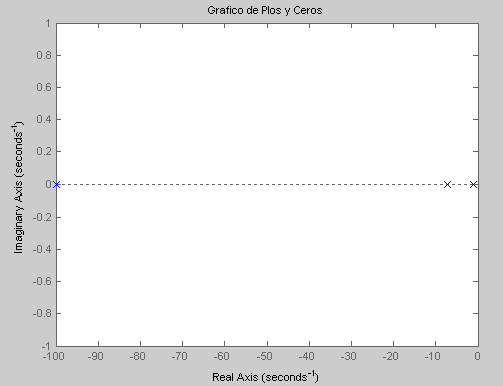
\includegraphics[width=0.7\linewidth]{cp1}}
	\caption{Gráfico de Polos y Ceros del Sistema.}
	\label{fig:cp1}
	\end{figure} 
Debido a que el sistema no posee polos en el origen, estamos en presencia de un sistema de tipo 0. El error de regimen permanente ante una señal de entrada escalón para estos casos se obtiene con la siguiente formula:
$$k_p=\lim\limits_{s\rightarrow 0}FT_{LA}(s) = 1$$
$$e_{ss}=\frac{1}{k_p+1}=\frac{1}{2}=0,5 $$
Es decir, que el error en estado estable del sistema es del 50\%.
\section{Funcion de Transferencia de Lazo Directo}
La funcion de transferencia de lazo directo es:
$$FT_{LD}=\frac{100}{0.001386s^2 + 0.1486 s + 1}$$
A continuacion se observa la salida de la funcion de transferencia de lazo directo ante una entrada de 10V. Se puede ver que llega al valor maximo que se espera del sistema de 1000lm.
  \begin{figure}[H] % Example image
	\center{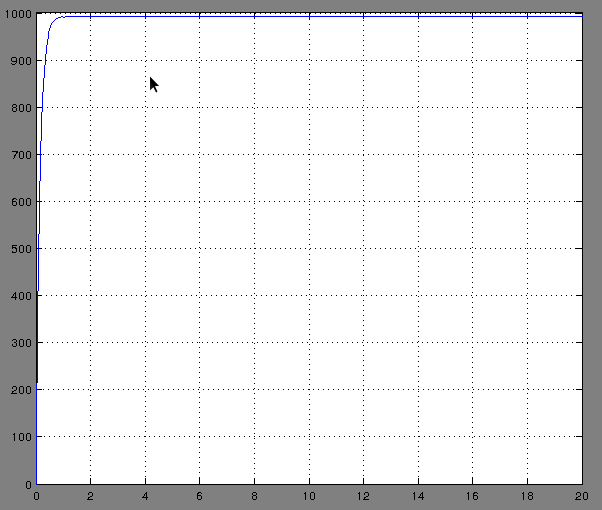
\includegraphics[width=0.7\linewidth]{resp_esc1}}
	\caption{Gráfico de la respuesta del sistema a la entrada escalón de 10V.}
	\label{fig:resp_esc1}
	\end{figure} 

\section{Funcion de Transferencia de Lazo Cerrado}
La funcion de transferencia de lazo cerrado es la siguiente:
$$FT_{LC}=\frac{FT_{Actuador} \times FT_{Driver} \times FT_{Planta}}{1+FT_{Actuador} \times FT_{Driver} \times FT_{Planta} \times FT_{Sensor}} $$
$$FT_{LC}=\frac{100*s+100}{0.001386s^3 + 0.15 s^2 + 1.149 s + 2}$$
Analisis de la funcion de transferencia:
\begin{table}[h!]
\centering
\caption{Esta tabla muestra los datos obtenidos de la separación zpk.}
\begin{tabular}{|ccccc|}
\hline 
 Ceros & Polos & Ganancia & Tipo \footnote{Debido a que el sistema no tiene polos al origen, el mismo es de tipo 0 (cero).} & Órden \tabularnewline
\hline 
\hline 
 -1 & -100,0863 & $7,2\times10^4$ & '0'(cero) & '3'(tres) \tabularnewline
 & -5,5332 & & &\tabularnewline
 & -2,6057 & & &\tabularnewline
\hline 
\end{tabular}
\end{table}
La funcion de transferencia de lazo cerrado en el modo \emph zpk es:
$$FT_{LC_{(ZPK)}}=\frac{7,2\times10^4(s+1)}{(s + 100.08)(s + 5,5)(s + 2,6)}$$
La ecuación caracteristica es:  
$$0.001386s^3 + 0.15 s^2 + 1.149 s + 2=0$$
Con el criterio de Routh-Hurwitz se determina que para tener un sistema estable, la ganancia k debe ser mayor a cero y menor que 61.08 (0 < k < 61.08).\\
\begin{table}[h!]
\centering
\caption{Aplicacion del criterio de Routh-Hurwitz, para analizar la estabilidad del sistema:}
\begin{tabular}{|c|c|c|}
\hline 
s3 & 0,001386 & 1,149\tabularnewline
\hline 
s2 & 0,15 & 2{*}k\tabularnewline
\hline 
s1 & 1,13-0,0185{*}k & 0\tabularnewline
\hline 
s0 & 2{*}k & \tabularnewline
\hline 
\end{tabular}
\end{table}

A continuacion se muestra el grafico de polos y ceros del sistema:\\

  \begin{figure}[H] % Example image
	\center{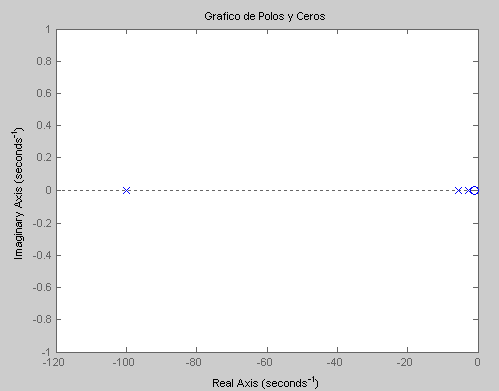
\includegraphics[width=0.7\linewidth]{cp2}}
	\caption{Gráfico de Polos y Ceros del Sistema.}
	\label{fig:cp2}
	\end{figure} 
	
Los polos dominantes del sistema son el 2.6 y 5.33, debido a que son los más cercanos al eje imaginario, y la distancia entre ellos es chica.\\
Respuesta de la funcion de transferencia de lazo cerrado a una señal de entrada escalón de 10V:

  \begin{figure}[H] % Example image
	\center{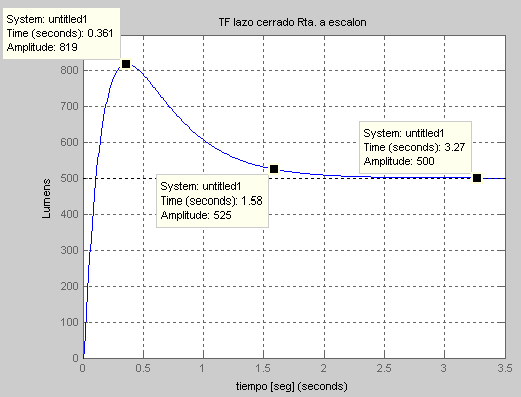
\includegraphics[width=0.7\linewidth]{resp_esc2}}
	\caption{Respuesta de la funcion de transferencia de lazo cerrado a una señal de entrada escalón de 10V.}
	\label{fig:resp_esc2}
	\end{figure} 

De la grafica se puede observar un sobrepasamiento aproximado de 320lm. El tiempo de aesntamiento es de 1.58 segundos. Y el error de estado estable es del 50\% ya que el sistema fue estimulado con un entrada de 10V, para la cual corresponderia una salida de 1000lm.\\
Respuesta de la funcion de transferencia a lazo cerrado ante una señal de entrada tipo rampa:

  \begin{figure}[H] % Example image
	\center{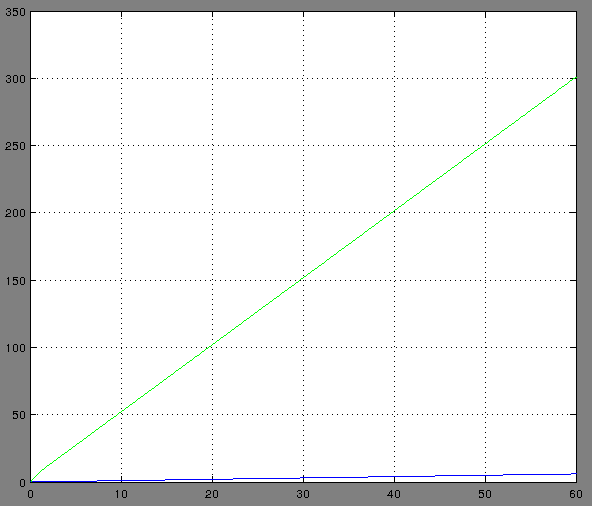
\includegraphics[width=0.7\linewidth]{resp_rampa1}}
	\caption{Respuesta de la funcion de transferencia a lazo cerrado ante una señal de entrada tipo rampa.}
	\label{fig:resp_rampa1}
	\end{figure} 

En la grafica se tiene en azul la entrada del sistema que tiene una pendiente de 0.1V, aproximando la variacion que puede producirse en la luminosidad debido al paso de una nube. Se considera que en 60 segundos puede llegar a disminuir aproximadamente un 60\% de la luz. La entrada al cabo de 60 segundos llega a los 6V.
En verde se observa la salida del sistema ante la rampa. Se puede ver que el sistema hace una curva al inicio hasta que se estabiliza y de ahi en mas sigue incrementandose, manteniendo un error del 50\% respecto al valor que se desearia tener como salida. A los 60 segundos la rampa llego a los 6V. Y la salida del sistema deseada es de 600lm, en este caso se tienen 300lm, un 50\% del valor deseado.

\section{Lugar de Raíces}

Graficar el lugar de raices es una herramienta muy utilizada en los analisis de los sistemas de control. Con esta se puede determinar si el sistema es estable para cualquier ganancia, o para determinar los valores de ganancia para los que el sistema se mantiene estable:

  \begin{figure}[H] % Example image
	\center{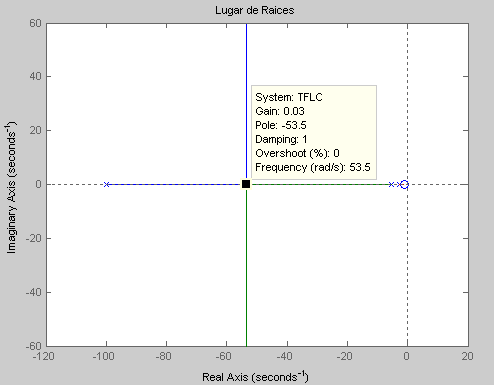
\includegraphics[width=0.7\linewidth]{LR1}}
	\caption{Gráfico del Lugar de Raices.}
	\label{fig:LR1}
	\end{figure} 

En el grafico se ve que al tener todo el lugar de raices en la parte real negativa del grafico el sistema sera estable para cualquier valor de ganancia mayor a cero, esto es para k>0.
El sistema será sobreamortiguado para valores de 0 a 0.03 y subamortiguado para valores de ganancia mayores a 0.03. Y sera criticamente amortiguado para k=0.03.\\
A continuación se muestran tres graficos para los distintios valores de k, para mostrar las distintas formas en las que reacciona el sistema.

Para k=0,02. Sistema sobreamortiguado.

  \begin{figure}[H] % Example image
	\center{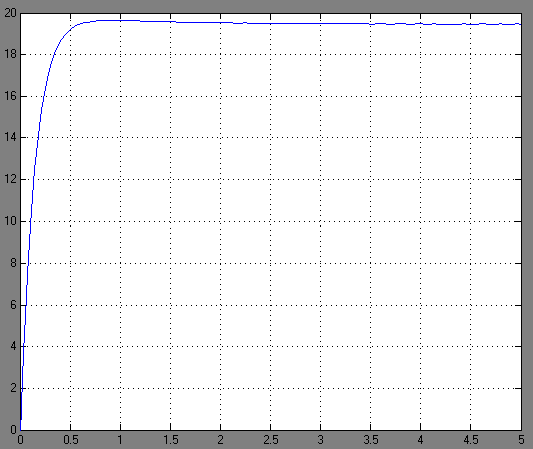
\includegraphics[width=0.7\linewidth]{resp_esc3}}
	\caption{Respuesta de la funcion de transferencia a lazo cerrado ante una señal de entrada tipo escalón para un k=0,02.}
	\label{fig:resp_esc3}
	\end{figure} 

Del grafico se observa que no hay sobrepaso, debido al sobreamortiguamiento, pero el valor en estado estable es menor a 20lm y es demasiado bajo. El error de estado estable aumento muchisimo, esto es debido a que la ganancia agregada es muy baja.

Para k=10. Sistema subamortiguado.

  \begin{figure}[H] % Example image
	\center{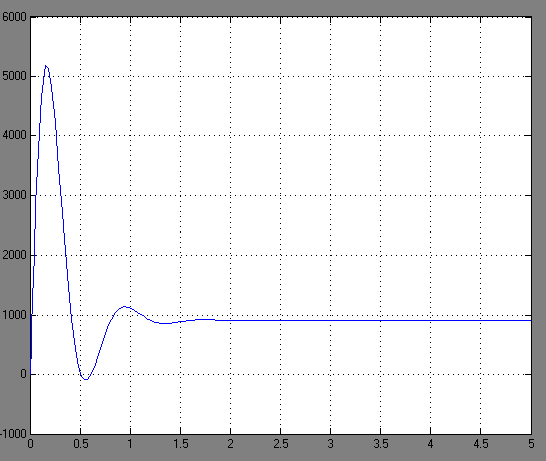
\includegraphics[width=0.7\linewidth]{resp_esc4}}
	\caption{Respuesta de la funcion de transferencia a lazo cerrado ante una señal de entrada tipo escalón para un k=10.}
	\label{fig:resp_esc4}
	\end{figure} 

Aqui, al contrario que en el caso sobreamortiguado, se puede ver que hay un sobrepaso muy elevado. Y debido a las oscilaciones que se observan se puede concluir que al sistema le cuesta llegar al valor de regimen permanente. Por otro lado el valor en regimen es proximo al deseado, es decir que se tiene un bajo error de estado estable.\\
Para k=0,03. Sistema Con amortiguamiento critico.\\

  \begin{figure}[H] % Example image
	\center{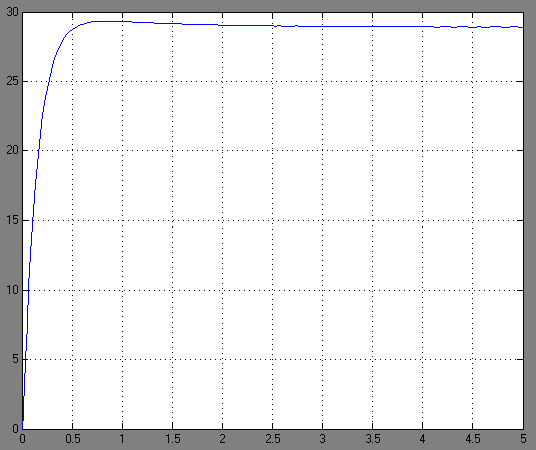
\includegraphics[width=0.7\linewidth]{resp_esc5}}
	\caption{Respuesta de la funcion de transferencia a lazo cerrado ante una señal de entrada tipo escalón para un k=0,03.}
	\label{fig:resp_esc5}
	\end{figure} 
	
Se tiene una salida sin sobrepaso, y un tiempo de asentamiento bajo, pero el error es muy grande, como en el caso de sobreamortiguamiento.
	
\section{Compensación}

\textsc{Requerimientos:}\\
-Error de estado estable: 5\%\\
-Tiempo de establecimiento: 2 segundos\\
-Sobrepaso: 5\%\\

Si bien la especificación indica un error de estado estable de 5\%, como máximo es conveniente tener el menor error posible, y como tenemos un sistema de tipo 0 se agregará un polo en el origen. Esto hará que el sistema pase a ser de tipo 1.
El integrador que se agrego al sistema es:$$\frac{0,1}{s}$$
Y al estimular el sistema con una entrada escalón de 10V se tiene un error de estado estable de 0\%.\\
	
  \begin{figure}[H] % Example image
	\center{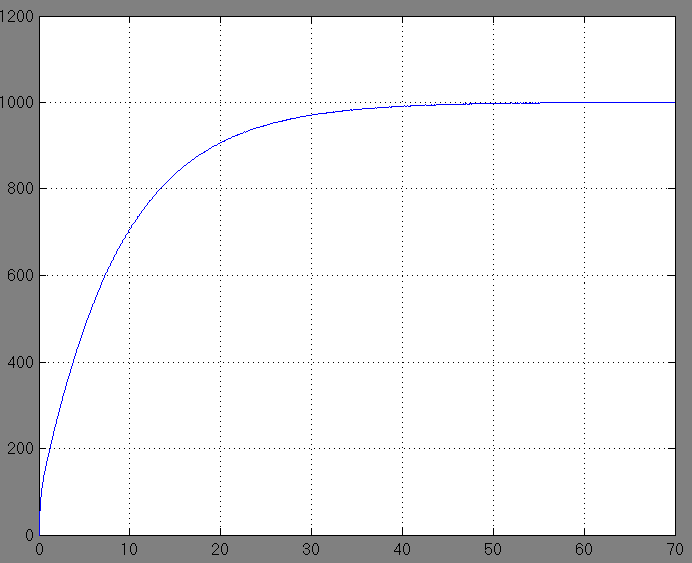
\includegraphics[width=0.7\linewidth]{resp_esc_int}}
	\caption{Respuesta de sistema con el integrador ante una señal de entrada escalón de 10V.}
	\label{fig:resp_esc_int}
	\end{figure} 

Como ya se dijo el error es 0\%, pero el tiempo de asentamiento se elevo considerablemente, ahora se tiene un tiempo aproximado de 40 segundo.

En el gráfico siguiente se muestra el nuevo lugar de raíces una vez agregado el integrador, y ademas se agrega una imagen ampliada en la región cercana al eje imaginario:\\

  \begin{figure}[H] % Example image
	\center{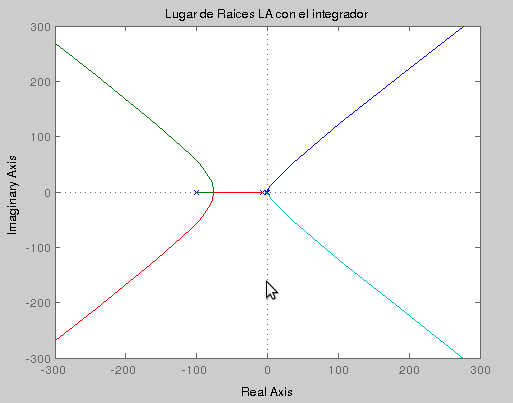
\includegraphics[width=0.7\linewidth]{LR2}}
	\caption{Grafico de lugar de Raices para el sistema con integrador.}
	\label{fig:LR2}
	\end{figure} 

	  \begin{figure}[H] % Example image
	\center{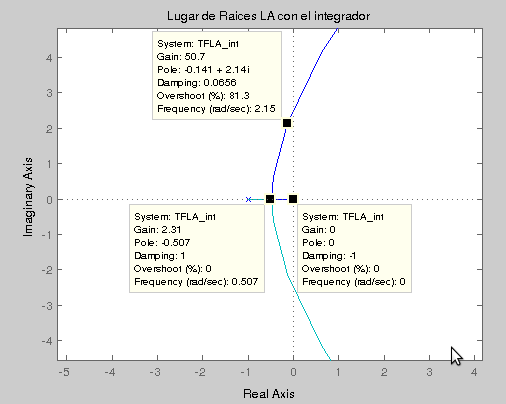
\includegraphics[width=0.7\linewidth]{LR3}}
	\caption{Acercamiento al orígen sobre el grafico de lugar de Raices para el sistema con integrador.}
	\label{fig:LR3}
	\end{figure} 
	
En esta ultima figura se ve que el sistema sera estable para $0<k<50.7$. Sera sobreamortiguado para $k<2.31$, subamortiguado para $2.31<k<50.7$. Y sera críticamente amortiguado para $k = 2.31$.\\
Para controlar este tiempo de establecimiento y llevarlo al valor especificado en los requerimientos debemos diseñar un compensador. Teniendo en cuenta el requerimiento de sobrepaso máximo se puede calcular el valor de $\zeta$:\\
$$0,05=e^{\frac{-\pi*\zeta}{\sqrt{1-\zeta^{2}}}}$$
Se obtiene un $\zeta$ de 0.707. Y teniendo en cuenta el requerimiento de tiempo de asentamiento calculamos el valor para la frecuencia Wn:
$$T_s=\frac{3}{\zeta*W_n} $$
$$W_n=\frac{3}{\zeta*T_s}=\frac{3}{0,707*2}$$
$$W_n=2,12$$
Con estos valores obtenidos se calculara el punto de diseño:
$$S = - \zeta*W_n + i*W_n*\sqrt{1-\zeta^2}$$
$$S = - 0,707*2,12 + i*2,12*\sqrt{1-0,707^2}$$
$$S = -1,5+1,5i$$
Como este punto de diseño no pertenece al lugar de raíces del sistema, y no puede ser alcanzado con una ganancia. Se procederá a diseñar un compensador que modifique el lugar de raíces para que contenga el punto de diseño.\\
Los polos de la función de transferencia de lazo abierto, incluyendo el integrador son:\\
\begin{center}
$P_0=0$\\
$P_1=-1$\\
$P_2=-7,22$\\
$P_3=-100$\\
\end{center}

Los ángulos aportados por cada polo respecto al punto de diseño son:\\
\begin{center}
$\angle_{P_0}=135\degree$\\
$\angle_{P_1}=108,43\degree$\\
$\angle_{P_2}=14,66\degree$\\
$\angle_{P_3}=0,87\degree$\\
\end{center}

%[AGREGAR LAS FORMULAS GENERICAS COMO EN EL OTRO TRABAJO, el que paso santiago]

Con estos ángulos se puede calcular el angulo del compensador:
$$\sum_{i}\angle_{C_i}=0$$
$$\sum_{j=0}^{3}\angle_{P_j}=135\degree+108,43\degree+14,66\degree+0.87\degree = +258.96\degree$$
$$\angle_{compensador} = 258.96\degree - (2k+1)180\degree$$

Tomando un k=0, ya que nos da el múltiplo mas cercano a 180°, se tiene:
$$\angle_{compensador} =78.96\degree$$
El compensador que debemos utilizar es un compensador en adelanto que nos permita disminuir el tiempo de establecimiento al valor de requerimiento.
A continuación se calcula el polo y el cero del compensador por el metodo de la bisectriz.
$$S = -1.5+1.5i$$
$$\angle_S=135\degree$$
$$\theta=180\degree-\angle_S$$
$$\theta=180\degree-135\degree$$
$$\theta=45\degree$$
%[FORMULAS DEL METODO DE LA BISECTRIZ]
$$Cero=-|S|\times\frac{cos(\frac{\theta+\phi}{2})}{cos(\frac{\theta-\phi}{2})}$$

$$Cero = -1.04$$

%[FORMULAS DEL METODO DE LA BISECTRIZ]
$$Polo=-|S|\times\frac{cos(\frac{\theta-\phi}{2})}{cos(\frac{\theta+\phi}{2})}$$

$$Polo = -4.32$$


%[EN CUADERNO ESTA EL DESARROLLO, no se si hará falta poner el desarrollo, quizás algo resumido]

$$Kc=25.9$$

%[ACA IRIA EL GRAFICO DEL COMPENSADOR]

\begin{table}[h!]
\centering
\caption{Cero, Polo y Ganancia del Compensador calculado.}
\begin{tabular}{c}
\hline
\hline 
$\displaystyle Cero = -1.04$\tabularnewline
$\displaystyle Polo = -4.32$\tabularnewline
$\displaystyle Kc=26$\tabularnewline
\hline
\hline
\end{tabular}
\end{table}

La función de transferencia resultante para el compensador PID es:
$$PID=2.59\times\frac{s+1.04}{s(s+4.32)}$$
Agregando el compensador al diagrama de bloques el sistema resulta:\\

  \begin{figure}[H] % Example image
	\center{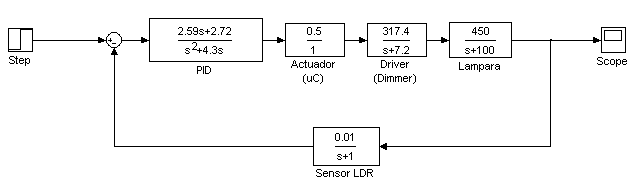
\includegraphics[width=0.7\linewidth]{diagrama3}}
	\caption{Diagrama de bloques con el Compensador PID.}
	\label{fig:diagrama}
	\end{figure} 
	
Las funciones de transferencia del sistema agregando el PID resultan:
$$FT_{LA_{PID}}=\frac{2,59s+2,72}{0,001386s^5+0,1559s^4+1,794s^3+5,939s^2+4,3s}$$
$$FT_{LA_{PID_{(ZPK)}}}=1868,7\times\frac{s+1,05}{(s+100)(s+7,23)(s+4,29)(s+1)s}$$
y a lazo cerrado
%$$FT_{LC_{PID}}=\frac{259s^2+531s+272}{0,001386s^5+0,1559s^4+1,794s^3+5,939s^2+6,89s+2,72}$$
%$$FT_{LC_{PID_{(ZPK)}}}=186807\times\frac{(s+1,05)(s+1)}{(s+100)(s+7,93)(s+0,9-0,26i)(s+0,9+0,26i)s}$$
EL lugar de raíces del sistema habiendo agregado el PID resulta:

  \begin{figure}[H] % Example image
	\center{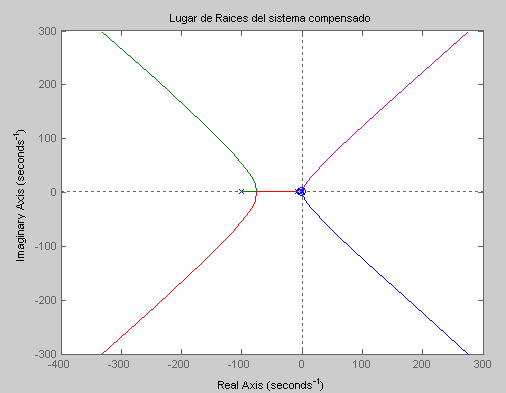
\includegraphics[width=0.7\linewidth]{LR_comp_1}}
	\caption{Gráfico del Lugar de Raices para el sistema con Compensador.}
	\label{fig:LR_comp_1}
	\end{figure} 
	
	  \begin{figure}[H] % Example image
	\center{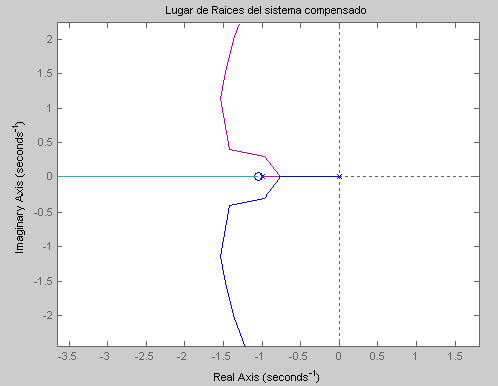
\includegraphics[width=0.7\linewidth]{LR_comp_2}}
	\caption{Gráfico del Lugar de Raices para el sistema con Compensador, con acercamiento en la zona cercana al eje imaginario.}
	\label{fig:LR_comp_2}
	\end{figure} 

A continuación se muestra la salida del sistema compensado para una entrada escalón de 10V:	
	
	  \begin{figure}[H] % Example image
	\center{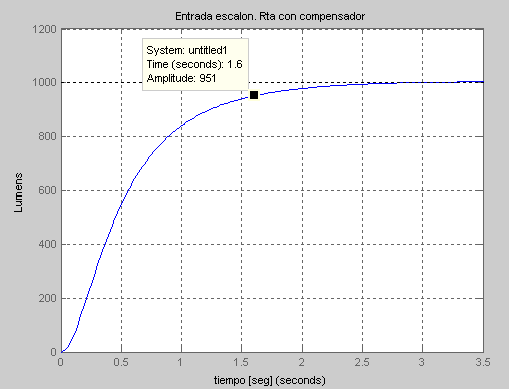
\includegraphics[width=0.7\linewidth]{resp_esc_comp1}}
	\caption{Respuesta del sistema compensado ante una señal de entrada escalón de 10V.}
	\label{fig:resp_esc_comp_1}
	\end{figure} 

Se puede ver que se cumplen los requerimientos pretendidos para el sistema. Éste no presenta sobrepaso y tampoco presenta error en estado estable, ya que la salida para un escalón de 10V de entrada es de 1000lm (es la deseada). Y el requerimiento respecto al tiempo de establecimiento de 2 segundos se cumple ya que el sistema se establece en 1.6 segundos.

La salida del sistema ante una rampa de pendiente 0,1, simulada durante 60 segundos llegando a 6V es:\\

	  \begin{figure}[H] % Example image
	\center{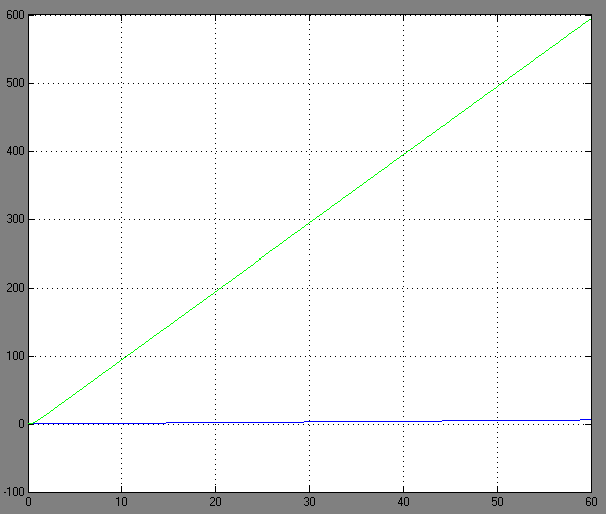
\includegraphics[width=0.7\linewidth]{resp_rampa_comp_1}}
	\caption{Respuesta del sistema compensado ante una señal de entrada tipo rampa de pendiente 0,1.}
	\label{fig:resp_rampa_comp1}
	\end{figure} 

En este gráfico se ve que el error del sistema es 0\%. Antes del compensador se tenia un error de 50\%, mientras que ahora ante la misma entrada se tienen los 600lm deseados.\\
\section{Respuesta del Sistema ante distintas Perturbaciones}

En esta sección se producirán distintas perturbaciones en la salida del sistema, para observar como responde el sistema ante las mismas. Como entrada del sistema, para todos los casos, se tendrá una señal escalón de 8V. Para esta entrada se espera tener una salida de 800lm.

El siguiere gráfico muestra la salida, al introducir una señal escalón de 100lm a la salida del sistema a los 5 segundos, luego de que se haya llegado al estado estable:\\

	  \begin{figure}[H] % Example image
	\center{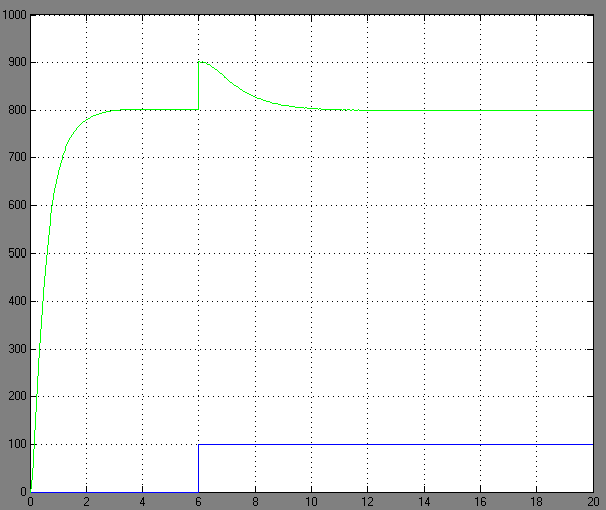
\includegraphics[width=0.7\linewidth]{ruido1}}
	\caption{Respuesta del sistema compensado ante una señal de ruido tipo escalón de 100lm inyectada en la salida una vez alcanzado el régimen.}
	\label{fig:ruido1}
	\end{figure} 

Se aprecia como el sistema se ve afectado, debido a que la entrada es repentina, pero luego de unos segundos logra superar esa perturbación, acomodando la salida al valor deseado de 800lm.\\
La siguiente perturbación corresponde a una rampa, con una pendiente de 20 lúmenes por segundo, introducida a los 5 segundo de comenzada la simulación. El sistema alcanzo su estado estable:\\

	  \begin{figure}[H] % Example image
	\center{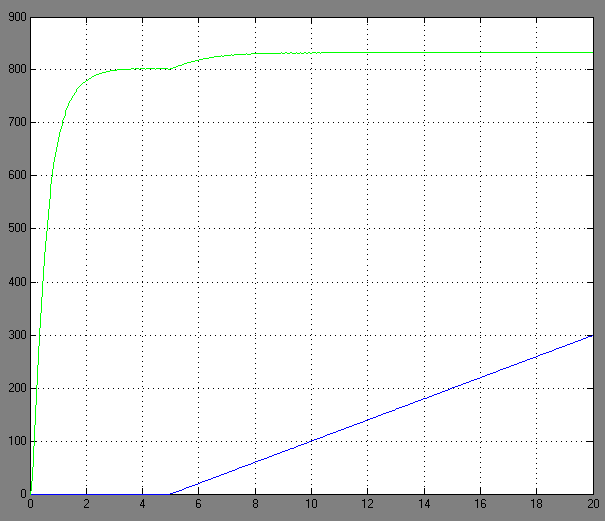
\includegraphics[width=0.7\linewidth]{ruido2}}
	\caption{Respuesta del sistema compensado ante una señal de ruido tipo rampa con pendiente de 20lm por segundo inyectada en la salida una vez alcanzado el régimen.}
	\label{fig:ruido2}
	\end{figure} 

El sistema no logra volver al valor deseado de 800lm, pero logra controlar la perturbación manteniendo un error de estado estable constante., y se mantiene en 830lm aproximadamente.\\
Por último se perturbará el sistema con una señal senoidal, con un frecuencia de 0.1Hz, y una amplitud de 200lm. Esta perturbación esta desde el inicio de la simulación:\\

	  \begin{figure}[H] % Example image
	\center{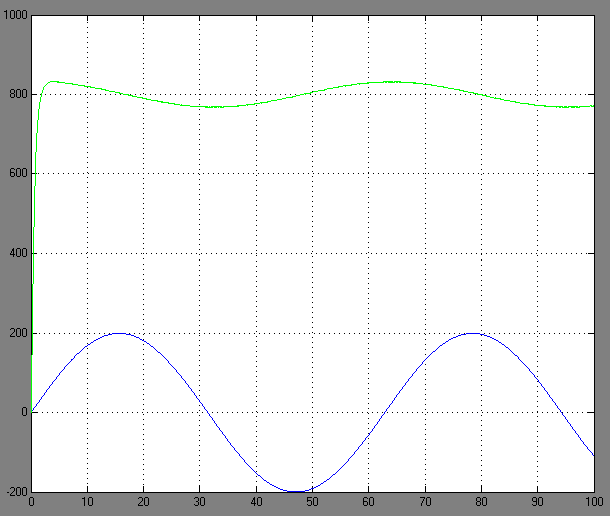
\includegraphics[width=0.7\linewidth]{ruido3}}
	\caption{Respuesta del sistema compensado ante una señal de ruido tipo senoidal de 0.1Hz inyectada en la salida.}
	\label{fig:ruido3}
	\end{figure}
	
Se puede ver como el sistema atenúa la amplitud de la perturbación, oscilando entre 770lm y 830lm, alrededor del valor deseado de 800lm.\\
Si se aumenta la frecuencia de oscilación el sistema ya no consigue controlarla. Se ha simulado el sistema con la misma señal de perturbación pero con una frecuencia de 1Hz. En este caso el sistema no es capaz de controlar esta perturbación. Pero para los propósitos de este trabajo esa frecuencia es elevada ya que es muy improbable que se produzcan variaciones tan rápidas en la luminosidad de un ambiente.
Ademas se ha simulado el sistema con la misma señal con una frecuencia mas baja, de 0.01Hz. El sistema ha sido capaz de controlarla y mantenerse en el valor deseado de 800lm, teniendo un error de estado estable de 0\%.\\

\section{Respuesta en Frecuencia}
\sloppy
La respuesta en régimen permanente de un sistema a señales sinusoidales en un rango de frecuencias es lo que se conoce como la respuesta en frecuencia del sistema.\\
El interés de tratar entradas sinusoidales está en que la respuesta del sistema a estas señales contiene información sobre la respuesta a señales más generales. De hecho, toda señal periódica puede descomponerse en una serie de senos y cosenos, por el Teorema de Fourier. Conociendo la respuesta del sistema a las componentes sinusoidales de la señal de entrada, puede reconstruirse por Fourier la señal de salida.\\
A continuación se muestra el Diagrama de Bode del Sistema en Lazo Abierto sin y con el compensador:\\

	\begin{figure}[H] % Example image
	\center{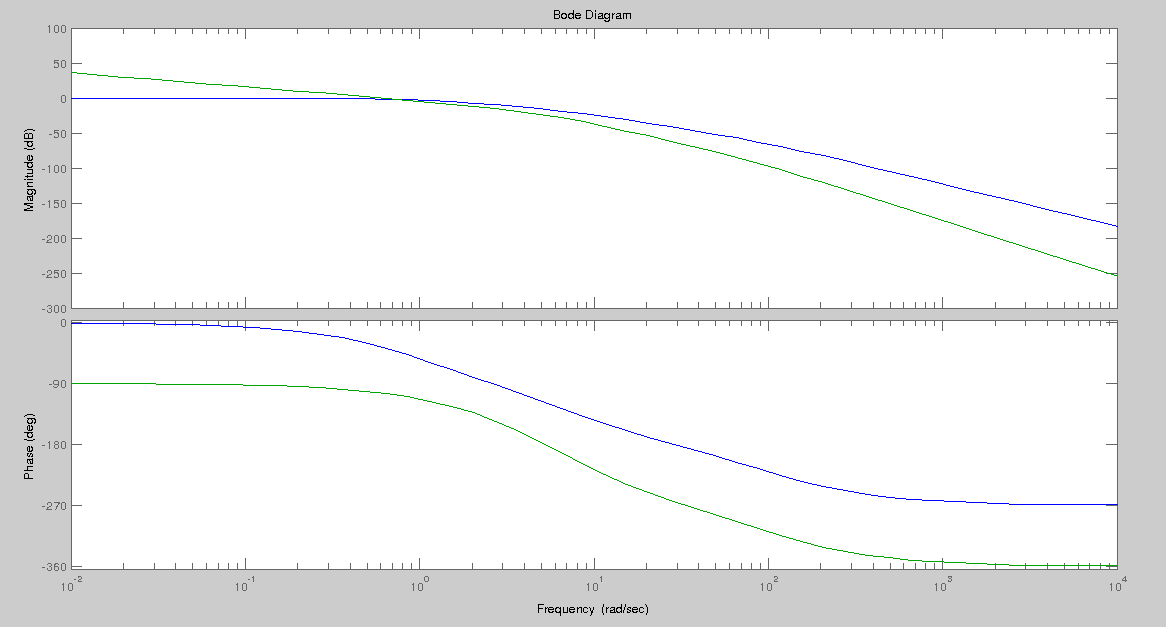
\includegraphics[width=\linewidth]{bode1}}
	\caption{Diagrama Bode de ambas funciones, en azul a Lazo Abierto sin Compensador
	y en verde con Compensador.}
	\label{fig:bode1}
	\end{figure}
	
Hay dos parámetros que miden la estabilidad relativa de un sistema de control:
\begin{itemize}
\item Margen de Fase.
\item Margen de Ganancia.
\end{itemize}

\textsc{Margen de Fase}

El margen de fase es la cantidad de atraso de fase adicional en la frecuencia de cruce de ganancia requerida para llevar el sistema al borde de la inestabilidad.\\
Sea $\omega_{FCGan}$ la frecuencia de cruce de ganancia es la frecuencia tal que hace que $|FT(j\omega_{FCGan})|=1\rightarrow 0dB$. Si $\phi(j\omega_{FCGan})$ es el ángulo del sistema de lazo abierto, entonces el margen de fase se define como:

$$M_{frec}=180\degree+\phi(j\omega_{FCGan})$$

\textsc{Margen de Ganancia}

El margen de ganancia es el recíproco de la magnitud $|G(j\omega)|$ en la frecuencia a la cual el ángulo de fase es -180° . Si $\omega_{FCFase}$ es esta frecuencia, entonces se define como:

$$M_{gan}=\frac{1}{|FT(j\omega_{FCFase})|}$$
En deciBeles:\\
$$M_{gan_{dB}}=20\times\log M_{gan}=-20\times\log|FT(j\omega_{FCFase})|$$

Para un sistema estable de fase mínima, el margen de ganancia indica cuánto puede incrementarse la ganancia antes de que el sistema se vuelva inestable. Para un sistema inestable, el margen de ganancia indica cuánto debe disminuir la ganancia para que el sistema se vuelva estable.

	\begin{figure}[H] % Example image
	\center{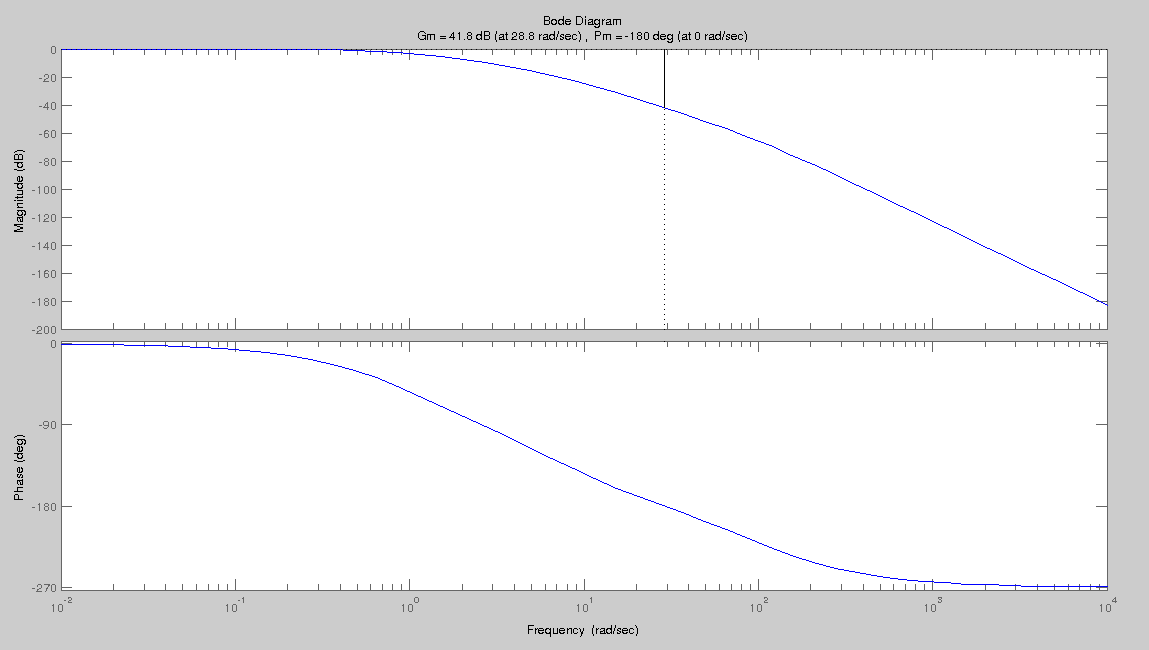
\includegraphics[width=\linewidth]{bode2}}
	\caption{Diagrama de Márgenes de la función de transferencia a lazo abierto sin compensador.}
	\label{fig:bode2}
	\end{figure}
	
	\begin{figure}[H] % Example image
	\center{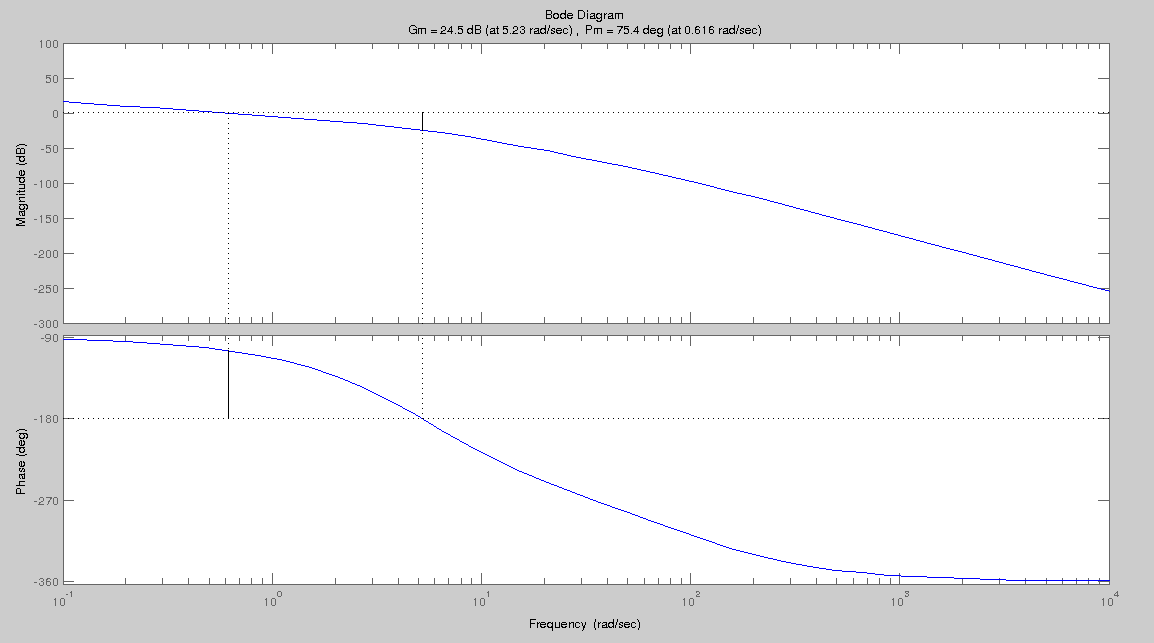
\includegraphics[width=\linewidth]{bode3}}
	\caption{Diagrama de Márgenes de la función de transferencia a lazo abierto con compensador.}
	\label{fig:bode3}
	\end{figure}
	
	\begin{figure}[H] % Example image
	\center{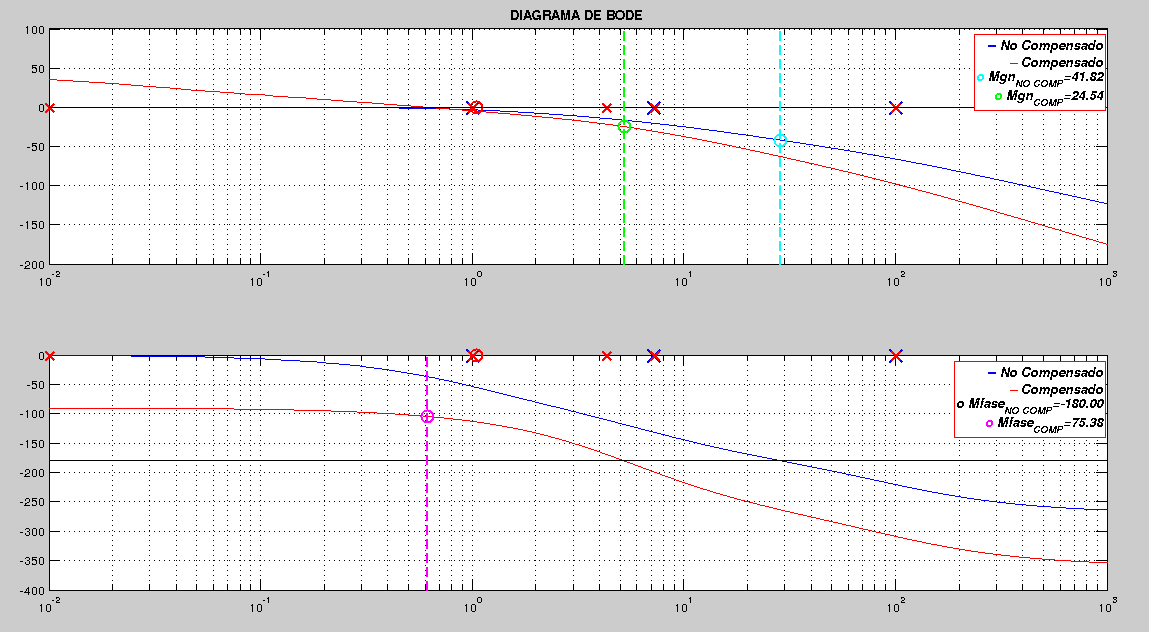
\includegraphics[width=\linewidth]{Bode_GIMP}}
	\caption{Diagrama de Bode con los márgenes, ceros y polos.}
	\label{fig:Bode_GIMP}
	\end{figure}

\begin{table}[h!]
\centering
\caption{Valores obtenidos del Análisis en Frecuencia.}
\begin{tabular}{|c|c|}
\hline
$LA_{NO COMP}$ & $LA_{COMPENSADO}$\tabularnewline
\hline
\hline 
$M_{gan}=41,82[dB]$ & $M_{gan}=24,54[dB]$\tabularnewline
\hline 
$M_{frec}=-180\degree $ & $M_{frec}=-45,38\degree $\tabularnewline
\hline 
$\omega_{FCGan}=0[\frac{rad}{seg}]$ & $\omega_{FCGan}=0[\frac{rad}{seg}]$\tabularnewline
\hline
\end{tabular}
\end{table}

Como puede observarse en los gráficos y más facilmente en Cuadro 5  los valores para los márgenes tanto de ganancia como el de fase acusan estabilidad para la version sin y con compensador de la función de transferencia de Lazo Abierto del Sistema.
En cuanto a la frecuencia de cruce de ganancia $\omega_{FCGan}$ se observa un desplazamiento positivo de 0,616 rad/seg por eso la disminución en el margen. 

\section{Variables de Estado}
La representación del sistema sin compensar con variables de estado es:\\
\center{
$\begin{cases}
\dot{x}=
\begin{bmatrix}
-107,21 & -721,5\\
1 & 0
\end{bmatrix}\times
\begin{bmatrix}
x_1\\
x_2
\end{bmatrix}+
\begin{bmatrix}
1\\
0
\end{bmatrix}\times
u \\
\\
y=1\times10^4\times
\begin{bmatrix}
0 & 7,21
\end{bmatrix}\times
\begin{bmatrix}
x_1\\
x_2
\end{bmatrix}+
\begin{bmatrix}
0
\end{bmatrix}\times
u
\end{cases}$
}\\
La representación del sistema compensado con variables de estado es:\\
\center{
$\begin{cases}
\dot{x}=1\times10^3\times
\begin{bmatrix}
-0,1 & -1,3 & -4,3 & -3,1 & 0\\
0,001 & 0 & 0 & 0 & 0\\
0 & 0,001 & 0 & 0 & 0\\
0 & 0 & 0,001 & 0 & 0\\
0 & 0 & 0 & 0,001 & 0
\end{bmatrix}\times
\begin{bmatrix}
x_1\\
x_2\\
x_3\\
x_4\\
x_5
\end{bmatrix}+
\begin{bmatrix}
x_1\\
x_2\\
x_3\\
x_4\\
x_5
\end{bmatrix}\times
u \\
\\
y=1\times10^3\times
\begin{bmatrix}
0 & 0 & 0 & 1,87 & 1,96
\end{bmatrix}\times
\begin{bmatrix}
x_1\\
x_2\\
x_3\\
x_4\\
x_5
\end{bmatrix}+
\begin{bmatrix}
0
\end{bmatrix}\times
u
\end{cases}$
}\\
\raggedright
\vspace*{1\baselineskip}
\textsc{Controlabilidad}\\
La controlabilidad de estados significa, usualmente, que es posible, mediante la inyección de entradas admisibles, cambiar los estados de cualquier valor inicial a cualquier valor final dentro de un intervalo de timepo.\\
Según Kalman un sistema es controlable si y sólo si la matriz \emph C tiene rango completo:
$$C=
\begin{bmatrix}
b & A\times b & A^2\times b & A^3\times b & ... & A^{(n-1)}\times b 
\end{bmatrix} $$

$$\det[C] \neq 0\;\;\footnote{Si la determinante de la matriz \emph C es distinta de cero entonces \emph C tiene rango completo}$$
Utilizando matlab se calculo la matriz de controlabilidad del sistema compensado:
$$
C=1\times10^8\times
\begin{bmatrix}
0 & 0 & 0 & -0,01 & 1,14\\
0 & 0 & 0 & 0 & -0,01\\
0 & 0 & 0 & 0 & 0\\
0 & 0 & 0 & 0 & 0\\
0 & 0 & 0 & 0 & 0
\end{bmatrix}
$$

Si bien la matriz parece ser casi todos ceros, esto es debido al redondeo realizado por matlab, a esta matriz se le calculo el rango con la funcion \verb+rank()+, el cual dio 5. En consecuencia se llega a que el sistema es \emph{Controlable}, esto implica que para un determinado rango de entradas admisibles, se va a poder alcanzar un valor de salida establecido.\\
\vspace*{1\baselineskip}
\textsc{Observabilidad}\\
La observabilidad de un sistema implica que conociendo los valores que toma \emph y se pueden conocer todos los valores de las variables de estado.\\
Según Kalman un sistema es observable si y sólo si la matriz \emph O tiene rango completo:\\
$$O=
\begin{bmatrix}
C^T\\
C^T\times A\\
C^T\times A^2\\
C^T\times A^3\\
...\\
C^T\times A^{(m-1)}
\end{bmatrix} $$

$$\det[O] \neq 0\;\;\footnote{Si la determinante de la matriz \emph C es distinta de cero entonces \emph O tiene rango completo}$$

Utilizando matlab se calculo la matriz de observabilidad del sistema compensado:
$$
O=1\times10^8\times
\begin{bmatrix}
0 & 0 & 0 & 0,001 & 0,002\\
0 & 0 & 0,002 & 0,002 & 0\\
0 & 0,002 & 0,002 & 0 & 0\\
0,002 & 0,002 & 0 & 0 & 0\\
-0,208 & -2,418 & -8,007 & -5,797 & 0
\end{bmatrix}
$$
En esta se puede observar que el rango de la matriz es de 5, se confirma haciendo uso de la función \verb+rank()+ de matlab. Esto implica que el sistema es \emph{Observable}, por lo que a partir de valores de salida del sistema se puede establecer el estado interno del sistema.
\section{Código Matlab}
%\begin{lstlisting}[language=Octave,caption=Codigo Fuente usado para el trabajo.]
%\end{lstlisting}
\lstinputlisting{trans_funct.m}%[caption=Codigo fuente principal Matlab.]
\vspace*{5\baselineskip}
\lstinputlisting{dibujar_Bode.m}%[caption=Codigo fuente funcion dibujar_Bode.]
\end{document}
